% Source: Code/camera-to-radar_labeller/system_overview.tex
% Description: Land vs.\ buoy ambiguity. The buoy and land mass have similar persistence values, but connected-component area thresholding separates them. The land mass spans 847 cells; the buoy spans 3.

\documentclass[border=4pt]{standalone}
\usepackage{amsmath,amssymb,amsfonts}
\usepackage{tikz}
\usepackage{xcolor}
\usetikzlibrary{arrows.meta,positioning,calc,patterns,decorations.markings,shapes.geometric,fit,backgrounds}

\definecolor{Garnet}{HTML}{73000A}
\definecolor{Rose}{HTML}{CC2E40}
\definecolor{Atlantic}{HTML}{466A9F}
\definecolor{Congaree}{HTML}{1F414D}
\definecolor{Horseshoe}{HTML}{65780B}
\definecolor{Grass}{HTML}{CED318}
\definecolor{Honeycomb}{HTML}{A49137}
\definecolor{Black90}{HTML}{363636}
\definecolor{Black70}{HTML}{5C5C5C}
\definecolor{Black50}{HTML}{A2A2A2}
\definecolor{Black30}{HTML}{C7C7C7}
\definecolor{Black10}{HTML}{ECECEC}
\definecolor{WarmGrey}{HTML}{676156}
\definecolor{Sandstorm}{HTML}{FFF2E3}

\tikzset{
    every node/.style={font=\small},
    sysblock/.style={
        draw=Congaree, fill=Congaree!10, thick,
        minimum width=2.2cm, minimum height=1cm,
        align=center, sharp corners,
        text=black
    },
    sysarrow/.style={
        -Stealth, thick, color=Garnet
    },
    timeblock/.style={
        draw=none, fill=#1, minimum height=0.5cm,
        sharp corners, text=white, font=\footnotesize\bfseries,
        inner sep=2pt
    },
    ppiblob/.style={
        fill=#1, sharp corners, minimum size=4pt, inner sep=0pt
    },
}

\begin{document}
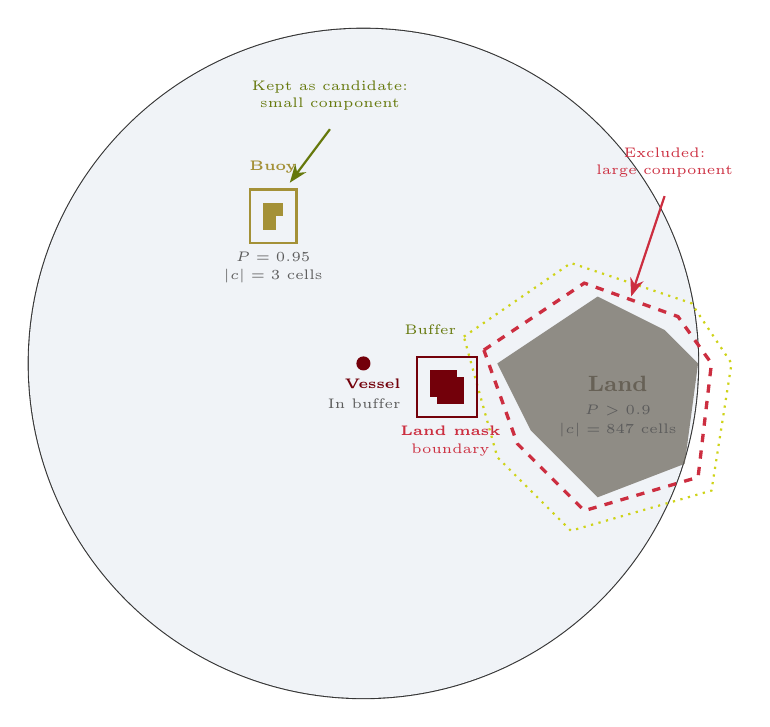
\begin{tikzpicture}[scale=0.85]
    % PPI circle
    \draw[thick, Black90] (0,0) circle (5cm);

    % Persistence map background (water = low persistence)
    \fill[Atlantic!8] (0,0) circle (5cm);

    % Land mass with high persistence
    \fill[WarmGrey, opacity=0.7] (2,0) -- (3.5,1) -- (4.5,0.5) -- (5,0) -- (4.8,-1.5) -- (3.5,-2) -- (2.5,-1) -- cycle;
    \node[font=\footnotesize\bfseries, text=WarmGrey] at (3.8,-0.3) {Land};
    \node[font=\tiny, text=Black70] at (3.8,-0.7) {$P > 0.9$};
    \node[font=\tiny, text=Black70] at (3.8,-1.0) {$|c| = 847$ cells};

    % Land mask boundary
    \draw[Rose, very thick, dashed] (1.8,0.2) -- (3.3,1.2) -- (4.7,0.7) -- (5.2,0) -- (5.0,-1.7) -- (3.3,-2.2) -- (2.3,-1.2) -- cycle;
    \node[font=\tiny\bfseries, text=Rose] at (1.3,-1.0) {Land mask};
    \node[font=\tiny, text=Rose] at (1.3,-1.3) {boundary};

    % Buffer zone
    \draw[Grass, thick, dotted] (1.5,0.4) -- (3.1,1.5) -- (4.9,0.9) -- (5.5,0) -- (5.2,-1.9) -- (3.1,-2.5) -- (2.0,-1.4) -- cycle;
    \node[font=\tiny, text=Horseshoe] at (1.0,0.5) {Buffer};

    % Buoy at 500m (high persistence, small area)
    \fill[Honeycomb] (-1.5,2.0) rectangle (-1.3,2.2);
    \fill[Honeycomb] (-1.4,2.2) rectangle (-1.2,2.4);
    \fill[Honeycomb] (-1.5,2.2) rectangle (-1.3,2.4);
    \draw[Honeycomb, thick] (-1.7,1.8) rectangle (-1.0,2.6);
    \node[font=\tiny\bfseries, text=Honeycomb, above] at (-1.35,2.7) {Buoy};
    \node[font=\tiny, text=Black70] at (-1.35,1.6) {$P = 0.95$};
    \node[font=\tiny, text=Black70] at (-1.35,1.3) {$|c| = 3$ cells};

    % Vessel near shore
    \fill[Garnet] (1.0,-0.5) rectangle (1.4,-0.1);
    \fill[Garnet] (1.1,-0.6) rectangle (1.5,-0.2);
    \draw[Garnet, thick] (0.8,-0.8) rectangle (1.7,0.1);
    \node[font=\tiny\bfseries, text=Garnet, left] at (0.7,-0.3) {Vessel};
    \node[font=\tiny, text=Black70, left] at (0.7,-0.6) {In buffer};

    % Radar center
    \fill[Garnet] (0,0) circle (3pt);

    % Annotation arrows
    \draw[-Stealth, Horseshoe, thick] (-0.5,3.5) -- (-1.1,2.7);
    \node[font=\tiny, text=Horseshoe, align=center] at (-0.5,4.0) {Kept as candidate:\\small component};

    \draw[-Stealth, Rose, thick] (4.5,2.5) -- (4.0,1.0);
    \node[font=\tiny, text=Rose, align=center] at (4.5,3.0) {Excluded:\\large component};
\end{tikzpicture}
\end{document}
